\newpage
\appendix
\section{Anhang}
\label{sec:Latex}
\subsection{Vollständige Implementierung Gene Folding}
\label{subsec:DokHeadGli}
\begin{minted}{c++}
#include <iostream>
#include <vector>
#include <algorithm>

using namespace std;

//prepossessing of a string to compute the length of even palindromes
string preString(string& str){
    string preStr = "#";    
    for(char c : str){
        preStr += c;
        preStr += '#';
    }    
    return preStr;
}

//computes the palindrome length for each char as center of the palindrome
vector<int> manacherAlgorithm(string& str){
    vector<int> lengths(str.length(),0);
    int c=0, r=0;
    for(int i=0; i<str.length(); i++){
        int mirror = 2*c-i;
        if(i<r){
            lengths[i] = min(r-i, lengths[mirror]);
        }
        int right = i+(1+lengths[i]);
        int left = i-(1+lengths[i]);
        while(left>=0 && right<str.length() && str[right] == str[left]){
            lengths[i]++;
            right++;
            left--;
        }
        if(i+lengths[i]>r){
            c = i;
            r = i+lengths[i];
        }
    }
    return lengths;
}

//computes the maximum prefix-palindrome index
int maxCut(vector<int>& lengths, string& str){
    int max=0;
    vector<int> lengths2 = lengths;
    for(int i=2; i<=(lengths2.size()); i+=2){
        if((lengths2[i]>0 && lengths2[i] == i) || lengths2[i]+max >= i){
            max = i;
        }
    }
    return max;
}

int main()
{   
    string input;
    cin >> input;
    
    //prefix
    string preStr = preString(input);
    vector<int> result = manacherAlgorithm(preStr);
    int prefixMax = maxCut(result, input);

    //suffix
    preStr = preStr.substr(prefixMax, preStr.length());
    vector<int> result2 = manacherAlgorithm(preStr);
    reverse(result2.begin(), result2.end());
    input = input.substr(prefixMax/2,input.length()-1);
    int suffixMax = prefixMax + result2.size()-maxCut(result2, input)-1;

    //computes the chars of the remaining string
    int res = ((suffixMax)-(prefixMax))/2;
    cout << res << endl;
    return 0;
}
\end{minted}
%
\subsection{Testskript Gene Folding}
\label{subsec:TextBefehle}
\begin{minted}{python}
import os
import subprocess
import time

cpp_program = "C:\\Users\\morit\\effiziente-algorithmen\\Gene Folding\\mainfinal.exe"
input_folder = "C:\\Users\\morit\\Desktop\\D-genefolding"
output_folder = "C:\\Users\\morit\\Desktop\\Laufzeit_GeneFolding"
output_file = "C:\\Users\\morit\\Desktop\\runtimes.txt"

with open(output_file, "w") as runtime_file:
    for filename in os.listdir(input_folder):
        if filename.endswith(".in"):
            input_path = os.path.join(input_folder, filename)
            ans_path = os.path.join(input_folder, filename.replace(".in", ".ans"))

            with open(input_path, "r") as file:
                input_string = file.read()

            start_time_case = time.time()

            result = 
            subprocess.run([cpp_program], input=input_string.encode(), 
            text=False, capture_output=True)

            end_time_case = time.time()
            duration_case = end_time_case - start_time_case

            input_length = len(input_string)

            cpp_output = result.stdout.decode()

            with open(ans_path, "r") as out_file:
                expected_output = out_file.read()

            is_correct = cpp_output.strip() == expected_output.strip()

            runtime_file.write(f"File: {filename}\n")
            runtime_file.write(f"Input Length: {input_length}\n")
            runtime_file.write(f"Result: {cpp_output}\n")
            runtime_file.write(f"Expected: {expected_output}\n")
            runtime_file.write(f"Correct: {is_correct}\n")
            runtime_file.write(f"Duration: {duration_case} seconds\n\n")

\end{minted}
%
\subsection{Testergebnisse Gene Folding}
\label{subsec:Mathematik}
\afterpage{%NEUE
\centering%NEUE
\begin{tabular}[h]{c|c|c|c|c|c}
     \textbf{Inputfile} & \textbf{Duration (s)} & \textbf{Correct?} & \textbf{Inputfile} & \textbf{Duration (s)} & \textbf{Correct?} \\
     \hline
     sample-1.in & 0.06543 & yes & sample-2.in & 0.01583 & yes \\
     secret-001.in & 0.11616 & yes & secret-002.in & 0.62825 & yes \\
     secret-003.in & 0.01526 & yes & secret-004.in & 0.02655 & yes \\
     secret-005.in & 0.01907 & yes & secret-006.in & 0.01897 & yes \\
     secret-007.in & 0.01834 & yes & secret-008.in & 0.01410 & yes \\
     secret-009.in & 0.01492 & yes & secret-010.in & 0.75532 & yes \\
     secret-011.in & 0.60981 & yes & secret-012.in & 0.62144 & yes \\
     secret-013.in & 0.55981 & yes & secret-014.in & 0.64379 & yes \\
     secret-015.in & 0.76912 & yes & secret-016.in & 0.75671 & yes \\
     secret-017.in & 0.75874 & yes & secret-018.in & 0.71544 & yes \\
     secret-019.in & 0.01570 & yes & secret-020.in & 0.01893 & yes \\
     secret-021.in & 0.01506 & yes & secret-022.in & 0.02276 & yes \\
     secret-023.in & 0.01576 & yes & secret-024.in & 0.01559 & yes \\
     secret-025.in & 0.01548 & yes & secret-026.in & 0.01602 & yes \\
     secret-027.in & 0.01517 & yes & secret-028.in & 0.02377 & yes \\
     secret-029.in & 0.02564 & yes & secret-030.in & 0.02036 & yes \\
     secret-031.in & 0.02834 & yes & secret-032.in & 0.02609 & yes \\
     secret-033.in & 0.01941 & yes & secret-034.in & 0.02104 & yes \\
     secret-035.in & 0.01787 & yes & secret-036.in & 0.03192 & yes \\
     secret-037.in & 0.02149 & yes & secret-038.in & 0.02726 & yes \\
     secret-039.in & 0.01929 & yes & secret-040.in & 0.02921 & yes \\
     secret-041.in & 0.02690 & yes & secret-042.in & 0.03223 & yes \\
     secret-043.in & 0.02542 & yes & secret-044.in & 0.04140 & yes \\
     secret-045.in & 0.02114 & yes & secret-046.in & 0.02085 & yes \\
     secret-047.in & 0.02565 & yes & secret-048.in & 0.03940 & yes \\
     secret-049.in & 0.02083 & yes & secret-050.in & 0.01802 & yes \\
     secret-051.in & 0.02347 & yes & secret-052.in & 0.02402 & yes \\
     secret-053.in & 0.01463 & yes & secret-054.in & 0.02247 & yes \\
     secret-055.in & 0.01695 & yes & secret-056.in & 0.02846 & yes \\
     secret-057.in & 0.02556 & yes & secret-058.in & 0.02624 & yes \\
     secret-059.in & 0.02466 & yes & secret-060.in & 0.02533 & yes \\
     secret-061.in & 0.02245 & yes & secret-062.in & 0.02739 & yes \\
     secret-063.in & 0.02937 & yes & secret-064.in & 0.01963 & yes \\
     secret-065.in & 0.85391 & yes & secret-066.in & 0.51321 & yes \\
     secret-067.in & 0.48282 & yes & secret-068.in & 0.48664 & yes \\
     secret-069.in & 0.50982 & yes & secret-070.in & 0.57523 & yes \\
     secret-071.in & 0.58711 & yes & secret-072.in & 0.67772 & yes \\
     secret-073.in & 0.49654 & yes & secret-074.in & 0.59495 & yes \\
     secret-075.in & 0.59470 & yes & secret-076.in & 0.51979 & yes \\
     secret-077.in & 0.59301 & yes & secret-078.in & 0.64789 & yes \\
     secret-079.in & 0.52325 & yes \\
\end{tabular}
\clearpage%NEUE
}
%
\subsection{Vollständige Implementierung A Safe Bet}
\label{subsec:DokHeadGli}
\begin{minted}{c++}
#include <iostream>
#include <vector>
#include <algorithm>
#include <stdio.h>
#include <set>
#include <string.h>

using namespace std;

//possible directions for the laser beam
#define N 0
#define E 1
#define S 2
#define W 3
#define MAX 2000000

int r, c, tree[MAX], lowestX = 1000000000, lowestY = 1000000000;
bool without;
typedef pair<int,int> p;
typedef long long int big;

set<p> rows[MAX];
set<p> columns[MAX];

//line objects for horizontal and vertical laser sections
class line{
    public:
        //start and end points of straight lines
        int xlow, ylow, xhigh, yhigh;
    
        line(int xl, int yl, int xh, int yh) : xlow(xl), ylow(yl), xhigh(xh), yhigh(yh){} 
};

//events for plane-sweep
class event{
    public:
        bool vertical;
        int value, low, high, add;

        event(bool ver, int val, int l, int h, int a) : vertical(ver), value(val), low(l),
        high(h), add(a){}

        bool operator < (const event &other)const{
            if(value != other.value){
                return value < other.value;
            }else if(add != other.add){
                return add > other.add;
            }else{
                return vertical > other.vertical;
            }
        }
};

//simulation of a laser beam as lines
void laserbeam(vector<line> &hori, vector<line> &verti, int x, int y, int dir){ 
    int nextX, nextY;
    bool next = true;

    while(next){
        //West
        if(dir == W){
            nextX = x;   
            nextY = 0;   //default
            auto it = rows[x].lower_bound({y,-1});

            if(it == rows[x].begin()){
                next = false;
            }else{
                it--;
                nextY = it->first;
                //next direction
                if(it->second){
                    dir = N;
                }else{
                    dir = S;
                }
            }
        //South 
        }else if(dir == S){
            nextX = r+1;   //default
            nextY = y;   
            auto it = columns[y].upper_bound({x,1000000000});

            if(it == columns[y].end()){
                next = false;
            }else{
                nextX = it->first;
                //next direction
                if(it->second){
                    dir = E;
                }else{
                    dir = W;
                }
            }
        //East           
        }else if(dir == E){
            nextX = x;   
            nextY = c+1;   //default
            auto it = rows[x].upper_bound({y,1000000000});

            if(it == rows[x].end()){
                next = false;
            }else{
                nextY = it->first;
                //next direction
                if(it->second){
                    dir = S;
                }else{
                    dir = N;
                }
            }
        //North
        }else if(dir == N){
            nextX = 0;   //default
            nextY = y;   
            auto it = columns[y].lower_bound({x,-1});

            if(it == columns[y].begin()){
                next = false;
            }else{
                it--;
                nextX = it->first;
                //next direction
                if(it->second){
                    dir = W;
                }else{
                    dir = E;
                }
            }            
        }

        if(nextX == x){
            hori.emplace_back(line{x, min(y, nextY)+1, x, max(y, nextY)-1});
        }else if(nextY == y){
            verti.emplace_back(line{min(x, nextX)+1, y, max(x, nextX)-1, y});
        }
        x = nextX;
        y = nextY;
    }
    //ends the laser in the detector
    if(x == r && y == c+1){
        without = true;
    }
}

//adds the value (= "add") to the given position and all subsequent positions (in the tree)
void update(int pos, int value){
    if(pos <= 0){
        return;
    }
    for(pos; pos < MAX; pos += (pos & -pos)){
        tree[pos] += value;
    }
}

//computes the prefix sum for a given position (from the tree)
big prefixSum(int pos){
    big result = 0;
    if(pos <= 0){
        return 0;
    }
    for(pos; pos>0; pos -= (pos & -pos)){
        result += tree[pos];
    }
    return result;
}

//computes the number of horizontal lines which cross the given section
big intervalSum(int left, int right){
    if(left>right){
        return 0;
    }
    return prefixSum(right) - prefixSum(left-1);
}

//computes all intersections for horizontal and vertical lines and stores the 
//lexicographically smallest
big intersections(vector<line> hori, vector<line> verti){
    memset(tree,0,sizeof tree);
    vector<event> e;
    big result = 0;

    //generate all events
    for(auto h : hori){
        e.emplace_back(false, h.ylow, h.xlow, h.xlow, 1);
        e.emplace_back(false, h.yhigh, h.xlow, h.xlow, -1);
    }
    for(auto v : verti){
        e.emplace_back(true, v.ylow, v.xlow, v.xhigh, -1);
    }
    sort(e.begin(), e.end());

    for(auto e1 : e){
        //vertical line
        if(e1.vertical){
            int low = e1.low;
            int high = e1.high;
            big inter = intervalSum(low, high);
            if(inter <= 0){
                continue;
            }
            //binary search to find precise intersection
            while(low < high){
                int mid = (low + high)/2;
                if(intervalSum(e1.low, mid) >= 1){
                    high = mid;
                }else{
                    low = mid+1;
                }
            }
            //keep track of the lexicographically smallest mirror
            if(low < lowestX){
                lowestX = low;
                lowestY = e1.value;
            }else if(low == lowestX && e1.value < lowestY){
                lowestY = e1.value;
            }            
            result += inter;

        //horizontal line
        }else{
            update(e1.low, e1.add);
        }
    }
    return result;
}

int main()
{   
    int curCase = 0;
    int m, n, x, y;

    while(scanf("%d%d%d%d", &r, &c, &m, &n) > 0){
        curCase++;

        //empty the sets rows and columns
        for(int i=0; i<=r+1; i++){
            rows[i].clear();
        }
        for(int i=0; i<=c+1; i++) {
            columns[i].clear();
        }

        //fill the rows and colums sets with "/"-mirrors (represented by 0)
        for(int i=0; i<m; i++){
            scanf("%d%d", &x, &y);
            rows[x].insert({y, 0});
            columns[y].insert({x, 0});
        }

        //fill the rows and colums sets with "\"-mirrors (represented by 1)
        for(int i=0; i<n; i++){
            scanf("%d%d", &x, &y);
            rows[x].insert({y, 1});
            columns[y].insert({x, 1});
        }

        //resets
        lowestX = 1000000, lowestY = 1000000;
        without = false;

        //laser starting at the top left of the grid (start point)
        vector<line> horiStart;
        vector<line> vertiStart;
        laserbeam(horiStart, vertiStart, 1, 0, E);

        //safe opens without inserting a mirror
        if(without){
            cout << "Case " << curCase << ": 0\n";
            continue;
        }

        //laser starting at the bottom right of the grid (end point)
        vector<line> horiEnd;
        vector<line> vertiEnd;
        laserbeam(horiEnd, vertiEnd, r, c+1, W);

        //count intersections
        big num = 0;
        num += intersections(horiStart, vertiEnd);
        num += intersections(horiEnd, vertiStart);

        //output
        if(num == 0){
            cout << "Case " << curCase << ": impossible\n";
        }else{
            cout << "Case " << curCase << ": " << num << " " << lowestX 
            << " " << lowestY << '\n';
        }
    }
    return 0;
}    
\end{minted}
%
\subsection{Testskript A Safe Bet}
\label{subsec:TextBefehle}
\begin{minted}{python}
import os
import subprocess
import time

cpp_program = "C:\\Users\\morit\\effiziente-algorithmen\\1287 A Safe Bet\\works.exe"
input_folder = "C:\\Users\\morit\\Desktop\\safe"
output_file = "C:\\Users\\morit\\Desktop\\runtimesSafe.txt"

with open(output_file, "w") as runtime_file:
    runtime_file.write("\\begin{longtable}{|l|l|}\n")
    runtime_file.write("\\hline\n")
    runtime_file.write("\\textbf{File} & \\textbf{Duration (s)} \\\\\n")
    runtime_file.write("\\hline\n")
    for filename in os.listdir(input_folder):
        if filename.endswith(".in"):
            input_path = os.path.join(input_folder, filename)

            with open(input_path, "r") as file:
                input_string = file.read()

            start_time_case = time.time()

            result = subprocess.run([cpp_program], input=input_string.encode(), text=False,
            capture_output=True)

            end_time_case = time.time()
            duration_case = end_time_case - start_time_case  # Sekunden

            runtime_file.write(f"{filename} & Duration: {duration_case:.4f} \\\\\n")
            runtime_file.write("\\hline\n")
    runtime_file.write("\\end{longtable}\n")    
\end{minted}
%
\subsection{Testergebnisse A Safe Bet}
\label{subsec:Mathematik}
\centering
\begin{tabular}[h]{c|c}
    \textbf{Inputfile} & \textbf{Duration (s)} \\
    \hline
    safe-001.in & Duration: 0.6788 \\
    safe-002.in & Duration: 0.2574 \\
    safe-003.in & Duration: 0.1923 \\
    safe-004.in & Duration: 0.1627 \\
    safe-005.in & Duration: 0.1697 \\
    safe-006.in & Duration: 0.2852 \\
    safe-007.in & Duration: 0.1860 \\
    safe-008.in & Duration: 0.1586 \\
    safe-009.in & Duration: 0.2234 \\
    safe-010.in & Duration: 0.2942 \\
    safe-011.in & Duration: 0.1864 \\
    safe-012.in & Duration: 0.2163 \\
    safe-013.in & Duration: 0.1959 \\
    safe-014.in & Duration: 0.1851 \\
    safe-015.in & Duration: 0.2584 \\
    safe-016.in & Duration: 1.1117 \\
    safe-017.in & Duration: 0.1507 \\
\end{tabular}
\begin{figure}[h]
    \centering
    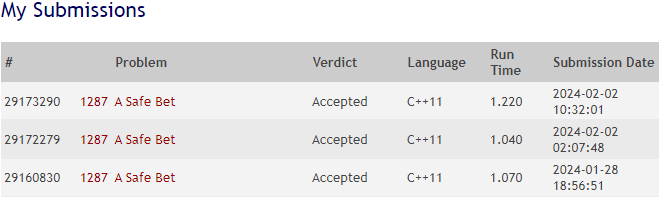
\includegraphics[width=14cm]{Bilder2/Abb6.PNG}
    \caption{Online-Judge Ausgabe.}
    \label{fig:enter-label}
\end{figure}
%
\begin{thebibliography}{99}
    \bibitem{bib:baeldung} Said Sryheni, Palindromic Substrings in O(N) with Manacher's Algorithm, \url{https://www.baeldung.com/cs/manachers-algorithm}, 8. Juni 2023.
    \bibitem{bib:boehm} Christian Böhm, Kapitel 6: Algorithmen der Computer-Geometrie, \url{https://www.dbs.ifi.lmu.de/Lehre/GIS/WS1112/Skript/GIS_WS11_06.pdf}, 2009.
    % Weitere Einträge
\end{thebibliography}
%